\begin{enumerate}[(a)]
	\item This is not a degree sequence of a graph, as there would be an odd
		number of vertices with odd degrees.
	\item Suppose this was the degree sequence of a graph. Then, by Havel-Hakimi
		theorem, so is $3,2,1,0,0,0$, and $1,0,0,0,0,-1$. But the last is clearly
		not a degree sequence, so the initial sequence is not either.
	\item This is the degree sequence of the graph \\
		\begin{tikzpicture}
			\draw
			(0:1) node {} -- (60:2) node {} -- (0:3) node {}
			(180:1) node {} -- (120:2) node {} -- (180:3) node {}
			(120:2) -- (60:2)
			(240:2) node {} -- (300:2) node {}
			;
		\end{tikzpicture}
	\item Iterations of Havel-Hakimi algorithm go as follows:
\subparagraph{0} 7,4,3,3,2,2,2,1,1,1
\subparagraph{1}   3,2,2,1,1,1,0,1,1
\subparagraph{2}     1,1,0,1,1,0,1,1 which is, of course (with rearrangement), the degree sequence of the graph of $3K_2$ with 2 isolated vertices added.
A graph with the original degree sequence is then \\
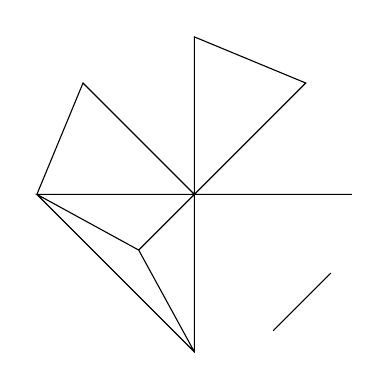
\begin{tikzpicture}
	\draw
	(0:2) node {} -- (0:0) node {} -- (45:2) node {} -- (90:2) node {} -- (0:0)
	(0:0) -- (135:2) node {} -- (180:2) node {} -- (270:2) node {} -- (0:0)
	(0:0) -- (225:1) node {} -- (180:2) -- (0:0)
	(225:1) -- (270:2)
	(300:2) node {} -- (330:2) node {}
	;
\end{tikzpicture}
\end{enumerate}
